\section{Performance comparison} 
\label{sec:performance_comparison}

\begin{figure}
	\centering
	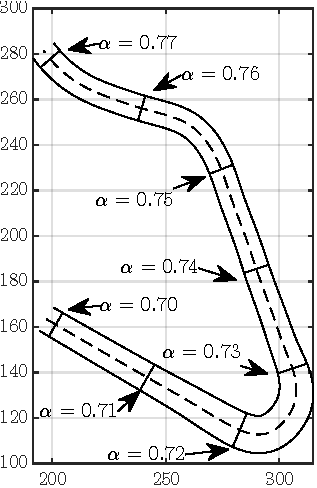
\includegraphics{Fig/track.pdf}
	\caption{Sector of the Catalunya circuit considered in the analysis, corresponding to the curvilinear abscissa interval $\left[0.70, 0.77\right]$. Checkpoints are indicated by labels and are uniformly spaced by $\De\al=0.01$. This sector includes two distinct corners: a low-speed turn from $\al = 0.72$ to $\al = 0.73$, and a high-speed turn from $\al = 0.75$ to $\al = 0.76$, allowing for the evaluation of vehicle behavior across different dynamic scenarios.}
	\label{fig:track}
\end{figure}

\subsection{Open loop parameters sensitivity}
\label{sec:ol_param_sensitivity}
In this section, we explore the open-loop approach to gain deeper insight into the influence of key parameters on the results. For this analysis, we consider optimizations in which only the track limit constraint is robustified. This choice is motivated by the fact that the effects of the track limit constraint are more visually evident compared to those of the friction limit constraint, thereby facilitating a more immediate understanding of their impact. 

The first parameter analyzed is the factor $\ga^\textrm{TLC}$, which multiplies the standard deviation of the constraint, $\sigma^\textrm{TLC}$, to determine the total back-off term $\be^\textrm{TLC}$. This parameter directly influences the probability of satisfying the track limit constraint: higher values of $\ga^\textrm{TLC}$ correspond to more conservative (i.e., robust) behavior. Specifically, $\ga^\textrm{TLC} = 0$ yields a satisfaction probability of 50\%, while $\ga^\textrm{TLC} = 3$ corresponds to 99\%. For the purposes of this analysis, we examine the effect of varying $\ga^\textrm{TLC}$ within this range. 

Setting $\ga^\textrm{TLC} = 0$ leads to the nominal solution. In this case, the back-off term $\be^\textrm{TLC}$ becomes zero, meaning that the constraint is not robustified and thus coincides with the original, non-robust formulation. 

Observing the left panel of Figure~\ref{fig:ol_sensitivities}, it is evident that the trajectories corresponding to configurations with lower values of $\ga^\textrm{TLC}$ tend to travel closer to the track boundaries. In contrast, the trajectory associated with $\ga^\textrm{TLC} = 3$---represented by the light green line---remains significantly farther from the edges.
This behavior is consistent with the increased conservativeness introduced by higher values of $\ga^\textrm{TLC}$, which amplify the back-off term $\be^\textrm{TLC}$ and thereby enforce a larger safety margin from the track limits.
Chasing a trajectory associated with a larger safety margin leads to higher sector times; spanning $\ga^\textrm{TLC}$ in the range $\left[0,3\right]$ results in sector times that vary from 12.135\,s to 13.162\,s.

\begin{figure}
	\centering
	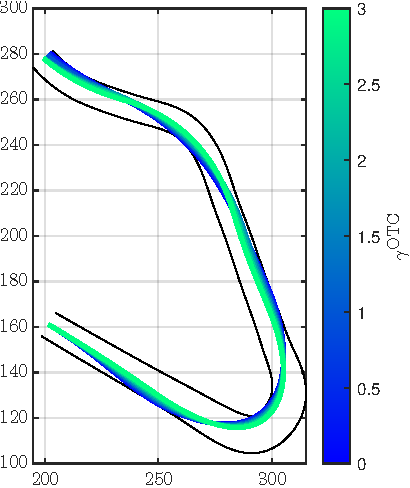
\includegraphics{Fig/gamma_sensitivity.pdf}
	\hfill
	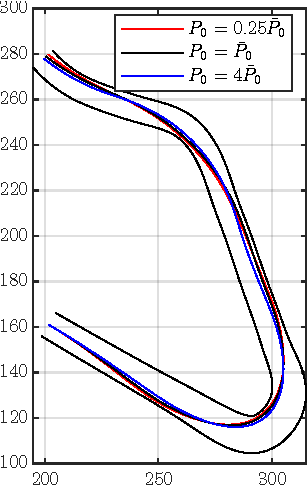
\includegraphics{Fig/Pzero_sensitivity.pdf}
	\caption{Effect of $\ga^\textrm{TLC}$ (left panel) and $P_0$ (right panel) on optimal trajectory. The parameter $\ga^\textrm{TLC}$ span in the range $\left[0,3\right]$ corresponding to a probability to meet the track limit constraint of 50\% and 99\%, respectively. In the left panel, in addition to the baseline value $\bar{\bP}_0$ (black line), two alternative values are considered: $\bP_0 = 4\bar{\bP}_0$ (blue line) and $\bP_0 = \frac{1}{4}\bar{\bP}_0$ (red line). These correspond, respectively, to doubling and halving the initial uncertainty associated with the state vector.}
	\label{fig:ol_sensitivities}
\end{figure}

The second parameter examined is the initial value of the covariance matrix, $\bP_0$. From this matrix, the standard deviation of each component of the mean state vector can be computed as:
\begin{equation}
	\sigma_i = \sqrt{e_i^T \bP_0 e_i},\label{eq:sigma_from_P}
\end{equation}
where $e_i$ is the unit vector with a 1 in the $i$-th position and zeros elsewhere. These standard deviations, $\sigma_i$, are used to evaluate the probability of the state vector remaining within a given interval. For example, considering the first element of the state vector, $\mu_1$, the interval $\left[\mu_1 - \sigma_1,\ \mu_1 + \sigma_1\right]$ corresponds to a 68\% probability of containing the true state, while the interval $\left[\mu_1 - 3\sigma_1,\ \mu_1 + 3\sigma_1\right]$ corresponds to approximately 99\%.

In addition to the baseline value $\bar{\bP}_0$, two alternative values are considered: $\bP_0 = 4\bar{\bP}_0$ and $\bP_0 = \frac{1}{4}\bar{\bP}_0$. These correspond, respectively, to doubling and halving the initial uncertainty associated with the state vector, as it's possible to verify from \eqref{eq:sigma_from_P}. 
For simplicity, a diagonal $\bar{\bP}_0$ has been chosen for this study. In this case, $\bar{\bP}_0$ is constructed by assigning the standard deviations of the elements of the state vector---collected in the vector $\bar{\boldsymbol{\sigma}}_0$---and placing their squared values along the diagonal. 
The values of $\bar{\boldsymbol{\sigma}}_0$ has been chosen accordingly to the range of variation of the associated variable. In particular, assuming the state vector is ordered as described in Section~\ref{sec:vehicle_model}, we selected $\bar{\boldsymbol{\sigma}}_0 = \left[0.1\,\textrm{m/s}, 0.01\,\textrm{m/s}, 0.01\,\textrm{rad/s}, 1\,\textrm{m}, 1\,\textrm{m}, 0.0175\,\textrm{rad}\right]^T$.

The results of the analysis conducted on this parameter are shown in the right panel of Figure~\ref{fig:ol_sensitivities} where the black line corresponds to the baseline, obtained setting $\bP_0 = \bar{\bP}_0$, while the red and the blue lines corresponds to configurations with $\bP_0 = \frac{1}{4}\bar{\bP}_0$ and $\bP_0 = 4\bar{\bP}_0$, respectively. 
Obviously, using a larger initial covariance matrix results in a greater covariance matrix after $H$ steps, which in turn leads to a higher back-off term. This is reflected in the blue line, which travels closer to the centerline w.r.t. the other two lines.

\subsection{Robustified constraints comparison}
It is of interest to analyze how a robustified constraint---or a combination of the two described in Sections~\ref{sec:FLC} and~\ref{sec:TLC}---influences the driving style. This analysis compares the not-robust trajectory, obtained without robustified constraints, with those resulting from a robustified track limit constraint (denoted as TLC), a robustified friction limit constraint (denoted as FLC), and a scenario where both constraints are robustified (denoted as TLC+FLC). All the optimization are obtained with the open-loop method described in Section~\ref{sec:open_loop_planning}, setting $H=4$, and $\ga^\textrm{TLC}=\ga^\textrm{FLC}=1.28$, corresponding to a 90\% probability of meeting both constraints. 

\begin{figure}
	\centering
	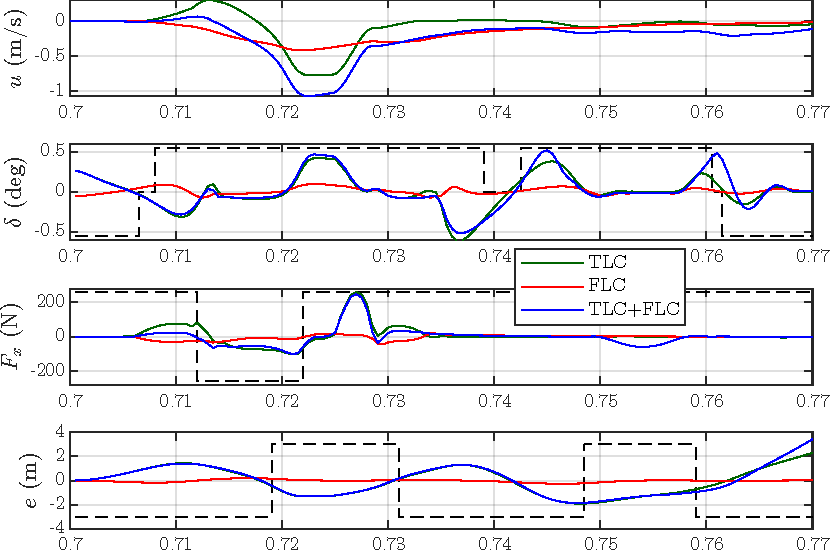
\includegraphics{Fig/ol_telemetries.pdf}
	\caption{Evolution of the longitudinal speed $\De u$, wheel steering angle $\De \de$, longitudinal force $\De F_x$, and lateral deviation $\De e$ are reported for three robustification scenarios: TLC (Track Limit Constraints), FLC (Friction Limit Constraint), and TLC+FLC (both constraints enforced concurrently). Each profile is shown relative to the baseline (nominal) trajectory to highlight the effect of each constraint-handling strategy. The dashed lines in the last three panels indicate the sign of the reference signal, allowing one to determine whether a positive variation with respect to the baseline corresponds to an increase or a decrease in the absolute value. This distinction is particularly important for quantities that depend on the direction of the turn, such as the wheel steering angle $\de$ and the lateral deviation $e$, while in the case of $F_x$, it indicates whether the vehicle is accelerating or braking.}
	\label{fig:ol_telemetries}
\end{figure}

Figure~\ref{fig:ol_telemetries} presents the variation of four signals with respect to the nominal trajectory, for the three previously mentioned cases. The panels display variations on the longitudinal speed $\De u$ (first panel), wheel steering angle $\De \de$ (second panel), total longitudinal force $\De F_x$ (third panel), and lateral deviation of the center of mass from the track centerline $\De e$ (fourth panel). Except for the $\De u$ panel, each plot includes dashed black lines that indicate the sign of the reference signal-whether it is positive, negative, or numerically zero. These sign indicators are represented as three distinct levels---high, zero, and low---corresponding to positive, zero, and negative values of the reference signal, respectively. The levels are scaled appropriately in each plot to ensure clarity of visualization.

From the first panel, it can be observed that all configurations maintain a lower mean value of the longitudinal speed compared to the reference trajectory, resulting in an increased sector time. Specifically, the configuration with the robustified TLC increases the sector time by 1.66\%, while the configuration with the robustified FLC and with both TLC and FLC robustified increase the sector time by 0.79\% and 2.57\%, respectively.
The two configurations incorporating the robustified track limit constraint (blue and green lines) exhibit, as expected, a significantly altered CoM trajectory. This behavior explains the higher longitudinal speed observed around $\al = 0.71$, which is followed by a sharp reduction. 

The second and fourth panels clearly show that the configurations with the robustified track limit constraint tend to follow a path closer to the centerline. In particular, for most of the sector, the variation in lateral displacement $\De e$ and the lateral displacement $e$ itself exhibit opposite signs, indicating a corrective behavior of the steering angle $\de$ that pulls the vehicle toward the centerline.

The third panel, which shows the variation of the total longitudinal force $\De F_x$, is consistent with the $\De u$ panel. In particular, the configurations with the robustified TLC exhibit a higher longitudinal force while approaching Turn 1, in the curvilinear abscissa interval $\al\in\left[0.707, 0.712\right]$, which results in a higher longitudinal speed. Subsequently, these two configurations apply a lower longitudinal force during braking compared to the nominal case, indicating more intense braking. This behavior explains the sharp reduction in longitudinal speed observed thereafter.

It can be interesting to notice that, in the third panel, only the configuration with both the constraints robustified (blue line) needs to reduce the longitudinal force during the high speed turn, in the curvilinear abscissa interval $\al\in\left[0.75, 0.76\right]$, to meet both the constraints. 
The vehicle constrained by the track limit condition is forced to follow a wider trajectory, which entails greater lateral acceleration and, consequently, a higher lateral force demand---resulting in increased tire utilization. Due to the limitations imposed by the robust friction limit constraint, it is necessary to reduce the available accelerating force.

After analyzing the variations of four key signals with respect to the nominal solution, we now turn our attention to the evaluation of axle saturation, which provides insight into how close each configuration operates to the tire grip limits.
Figure~\ref{fig:ol_saturation} presents the quantity $\left[ \left( \frac{X_j(\bx,\bu)}{\mu_{x,j}} \right)^2+ \left( \frac{Y_j(\bx,\bu)}{\mu_{y,j}}\right)^2\right]\frac{1}{Z_j^2(\bx,\bu)}$, where $j=1$ refers to the front axle (first panel) and $j=2$ the rear axle (second panel), plotted for the three previously introduced configurations (color-coded as before) and for the nominal solution (black dashed line). This quantity indicates how close each configuration operates to the friction limit; it equals 1 when the point $\left(X_j, Y_j\right)$ lies exactly on the friction ellipse defined by $Z_j$.

\begin{figure}
	\centering
	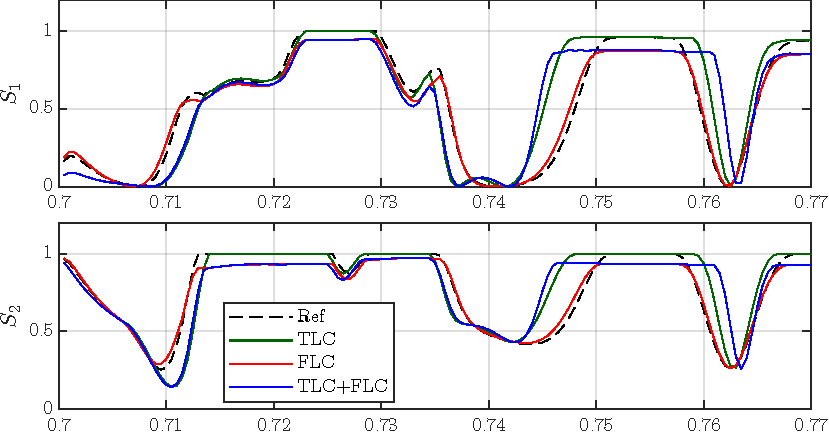
\includegraphics{Fig/ol_saturation.pdf}
	\caption{Tire usage for front axle (first panel) and rear axle (second panel) over curvilinear abscissa $\al$. The plotted lines represent the quantity $\left[ \left( \frac{X_j(\bx,\bu)}{\mu_{x,j}} \right)^2+ \left( \frac{Y_j(\bx,\bu)}{\mu_{y,j}}\right)^2\right]\frac{1}{Z_j^2(\bx,\bu)}$, where $j=1$ denotes the front axle and $j=2$ the rear axle. The dashed black line corresponds to the reference (nominal) configuration, while the green, red, and blue lines represent the robust configurations TLC, FLC, and TLC+FLC, respectively.}
	\label{fig:ol_saturation}
\end{figure}

As expected, the two configurations with the robustified friction limit constraint (red and blue lines) never reach a value of 1, due to the presence of the back-off term, which enforces a safety margin from the friction limit. 
From this plot, it can be observed that the configurations with the robustified track limit constraint (green and blue lines) follow significantly different trajectories compared to the nominal solution, resulting in distinct ground force demands. This behavior is noticeable in turn 1 and even more clearly in turn 2. Specifically, these two configurations begin to experience high axle loads approximately 12\,m before the nominal trajectory and sustain them for an additional 4.6\,m (TLC, green line) and 9.2\,m (TLC+FLC, blue line) beyond the nominal reference. 

\subsection{Simulations with noise realization}
This analysis aims to provide empirical validation of the robust trajectories obtained using the methods proposed in this work. For conciseness, the comparison is limited to a nominal trajectory and a trajectory computed using the closed-loop method with only the track limit constraint robustified.
An LQR controller, designed according to the procedure outlined in Section~\ref{sec:LQR}, is implemented along the nominal trajectory. In contrast, the robust trajectory is tracked using the controller directly obtained from the optimization process.

\begin{figure}
	\centering
	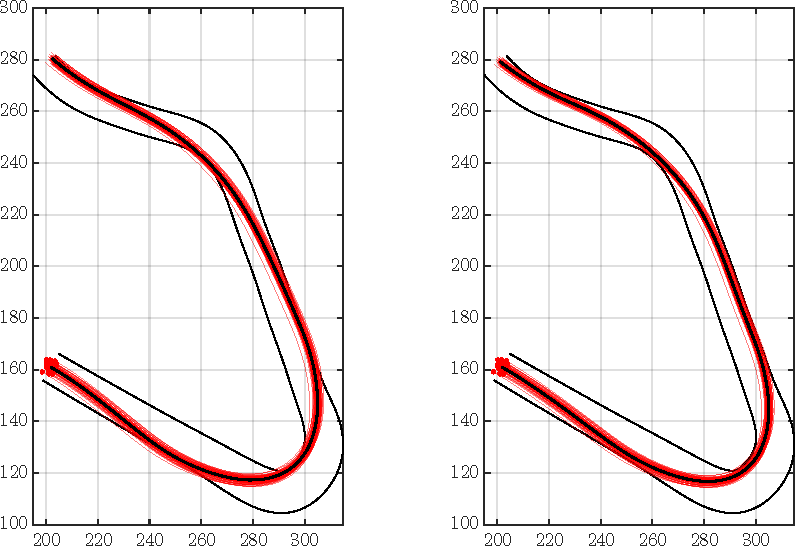
\includegraphics{Fig/olcl_traj_strings.pdf}
	\caption{Simulations with random initial conditions and Gaussian noise realizations. In the left panel, the reference trajectory is the non-robust one, tracked using an LQR controller designed around it. In the right panel, the reference is a robust trajectory obtained using the closed-loop optimization method, and it is tracked using the corresponding optimized controller produced by the same method.}
	\label{fig:traj_strings}
\end{figure}